% -*- latex -*-

In this chapter we capture the information acquired during the project that
is not directly related to the implementation of the Dax toolkit as
recorded in Chapters \ref{chap:Overview} and \ref{chap:Documentation}.

\section{Lessons Learned}

As with any research project, over the course of the work we made
discovers that taught us what does and does not work well. The publications
listed in the executive summary of this document report the major findings,
particularly the larger ones. Here we capture some smaller discoveries
that, although themselves not warranting their own publication, have
contributed to our understanding of developing a general purpose toolkit
for massively threaded visualization algorithms.

\subsection{Abandonment of Kernel Fusion}

In the original proposal for this project, we described a system that
builds a pipeline of operations, much like the VTK pipeline but with much
lighter-weight operations. The system would find chains of operations and
then group their execution together so that all operations would happen on
a single data element together. The main intention of this specialized form
of kernel fusion is to maximize the amount of execution happening per load
of the data.

As we attempted to implement such a system, we found the implementation was
more technically difficult than expected. Worse, the API for managing these
connections was extremely awkward in the sense that the it was difficult to
understand and difficult to use even if it was understood. Both the
underlying system and the API underwent several unsatisfactory redesigns.

Eventually, we decided that this extra complication in both interface and
implementation was not providing much. The Dax toolkit is already
structured in such a way as to encourage adding many instructions to a
minimal amount of data by coding through the worklet paradigm. Ultimately,
the optimization was doing nothing that a Dax user was not likely to be
doing herself.

This distraction stalled the toolkit development for several months. Once
we changed to a more imperative interface, development took off as is
evident with the plot of repository commits over time.

\noindent
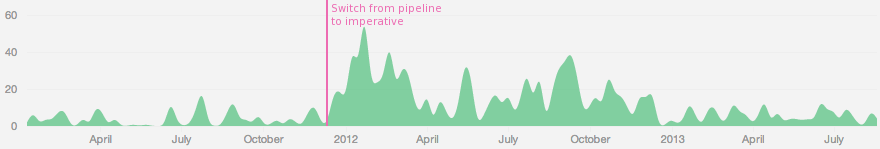
\includegraphics[width=\textwidth]{images/GitActivity}

\subsection{Explicit Memory Hierarchy}

The NVIDIA CUDA architecture has a very unique memory hierarchy. Cores are
grouped into streaming multiprocessor units that together access a local
``shared memory'' that is much faster than the global shared memory. Our
initial expectation was that we would gain significant performance
enhancement by explicitly managing these memory hierarchies.

However, early in the projects we made comparisons of the effect of memory
access when either explicitly loading data into these shared memory banks
or by simply allowing the GPU's caching mechanism to load the shared
memory. What we found was that the automatic caching mechanism generally
worked as well as our hand-tuned memory loading using knowledge about the
structure of the data and our access to it.

So, our conclusion is that allowing the caching mechanism is a good way to
populate the memory hierarchy while also realizing code that is simpler and
easier to maintain.

\subsection{Alternate Topology Data Structures}

Before designing algorithms within the Dax toolkit, we had to agree on a
data representation for our grid structures. Meshes like a uniform grid are
straightforward because their topology is implicit and there is nothing
much to capture. However, for more general unstructured combinations there
must be an explicit way to establish the shape of each cell and the
connections between them.

The data model used by VTK and many other software packages and
applications uses a vertex-cell model where an index array captures for
each cell the points that comprise the cell's vertices. The vertices for a
particular cell type follow a conventional order such as the CGNS
convention\lcite{CGNS}.

We also considered several alternate methods for representing meshes of
polyhedra. These included half-edge and winged-edge
structures\lcite{Kettner1998}, cellular data
structures\lcite{Alumbaugh2005}, and circular incident edge
lists\lcite{Levy2001}. All of these representations use a linked list of
indices that trace around the constituent elements of a cell.

The advantage of these structures is that the can capture some of the
incidence relationships that the vertex-cell model does not directly
capture. However, the disadvantage is that to build these structures, it
means finding these incidence relationships whether they are directly used
or not. Furthermore, when one mesh is derived from another mesh, these
relationships again have to be derived one from another. Another problem
with these mesh types is that they often require tracing links to find
information about the data structure, and following these linked lists is
often an inefficient operation on massively threaded processors.

Consequently, the Dax toolkit uses the traditional vertex-cell model to
represent its unstructured grids, as described in
Section~\ref{sec:GridStructures}. We have discovered a variety of sorting
techniques to find incidence relationships that are not explicitly captured
with the cell links.

\subsection{Data Transfer Time}

It is common knowledge that when using an accelerator like a GPU that you
should avoid transferring data to and from the accelerator like the
plague. This is because the speed of the bus between the host computer and
the accelerator device is orders of magnitude slower than accessing the
memory locally.

This advice is certainly true for something like rendering where a
repetitive operation must cycle at 20Hz or faster. It is also true for
small operations. For example, you cannot transfer data back and forth
every time a simple vector operation is performed. However, this advice can
lead you astray if taken too far.

We performed an informal investigation on the transfer time with respect to
the operating time of an algorithm within the Dax framework. What we find
is that for an operation that performs more than a trivial amount of
computation, the transfer time is insignificant. For example, the Marching
Cubes algorithm, which itself is not a huge amount of computation, still
spends two orders of magnitude more time in execution than in the total
time of transferring memory to and from the GPU as demonstrated in
Figure~\ref{fig:TransferVsExecution}.

\begin{figure}[htb]
  \centering
  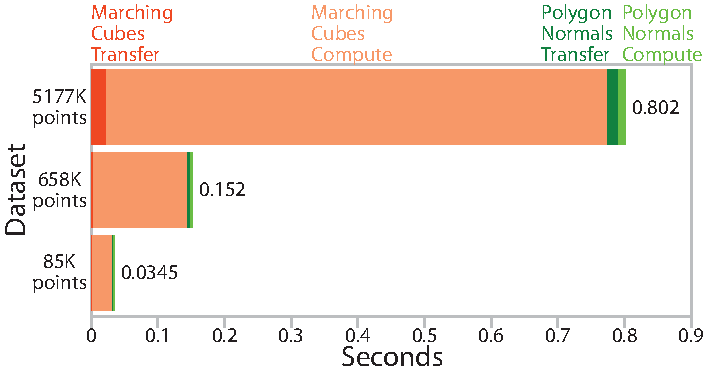
\includegraphics{images/TransferVsExecution}
  \caption{Comparison of execution time vs. transfer time.}
  \label{fig:TransferVsExecution}
\end{figure}

The importance of this finding is the simplification of integrating
algorithms in the Dax toolkit with other visualization systems like VTK and
ParaView. These are based on the visualization
pipeline\lcite{Moreland2013:TVCG}, which splits algorithms into individual
components. Although it would be possible to leave data on the GPU when
passing from one component to the next, it creates great difficulty in
managing the limited amount of memory available because there is no good
way to know what, if anything, will be required from one component to the
next.

A more tractable approach is to pull all data back to the host memory
before passing from one algorithm to the next. Compared to an algorithm
like Marching Cubes, the overhead is negligible. Even for very minor
operations like finding normals, the overhead does not get above a few
hundredths of a second. Since visualization pipelines typically do not get
very deep and are executed infrequently compared to other operations like
rendering, adding such an overhead is irrelevant in practice.

\section{Results}

The intention of the Dax project is to provide the generic infrastructure
to build visualization algorithms on. To demonstrate the infrastructure
currently implemented, we present to exemplary algorithms: threshold and
Marching Cubes.

\subsection{Threshold}

The threshold algorithm can be summarized as follows: For each cell in the
data set, find the points that form the cell and the corresponding scalar
field values for each of those points. If the scalar field values for all
the points are within the threshold range, then pass the cell and the
corresponding points to the output data set. Since points are often shared
between cells, we also avoid passing duplicate points in the output. This
ensures both that the representation of the output does not require more
space than needed and that the resultant data set is suitable for further
analysis if needed.

To implement the algorithm within the Dax framework, we need to map the
algorithm to multiple worklets. Based on the implementation by Lo
\etal\lcite{PISTON}, the thresholding operation can be characterized as the
following steps:

\begin{enumerate}
\item For every cell in the input data set, we need to first determine if it
  passes the threshold criteria. This can be implemented with a cell map
  worklet whose output is the number of cells it will create. In the case
  of threshold, this will be either 0 or 1 cell.
\item Once we have generated the count array, we need to determine how much
  space to allocate in the output and build indices from either input to
  output or output to input. This is a fairly common task in parallel
  programming, known as stream compaction. The Dax dispatcher performs this
  all internally before performing the following step.
\item For every cell that passes the threshold criteria, we need to
  generate a duplicate cell for the output. This operation is implemented
  inside of a generate topology worklet.
\item It is possible (and for threshold likely) that not all points in the
  output are referenced by a cell. The Dax dispatcher can remove unused
  points and compact the array; however, this step is optional.
\end{enumerate}

We demonstrate the threshold algorithm by running it on example supernova
simulation results on a $432^3$ uniform grid. In our first set of
experiments, we run a version of the algorithm that is isomorphic to what
VTK produces. The results of these experiments are summarized in
Figure~\ref{fig:TimingThresholdPointMask}.

\begin{figure}[htb]
  \centering
  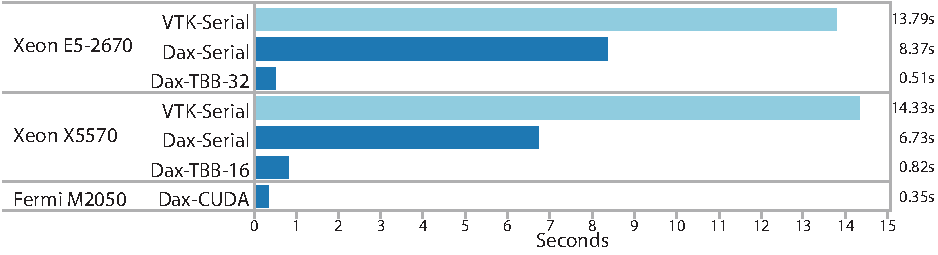
\includegraphics{images/TimingThresholdPointMask}
  \caption{Timing of threshold with output point masking.}
  \label{fig:TimingThresholdPointMask}
\end{figure}

We see that even when running Dax in serial, its threshold algorithm is
roughly twice as fast as the equivalent VTK algorithm. We attribute this
mostly to more efficient data manipulations in Dax. Furthermore, the Dax
parallel algorithm makes good use of multiple cores.

As previously stated, the final step of the generate topology method, where
unused points are removed, is optional. In our second set of experiments,
we run the algorithm on the same data set as before, but skip the
point-merging step. We compare the algorithm in Dax with an equivalent
algorithm from the PISTON project. Note, however, that we modified the
algorithm in PISTON to output cells equivalent to what Dax
produces. (Specifically, the original PISTON algorithm produces
quadrilaterals of the passed faces, and that was changed to produce the
hexahedra themselves. Our modified algorithm runs faster than the original
because it produces smaller arrays.) The results of these experiments are
summarized in Figure~\ref{fig:TimingThresholdNoPointMask}.

\begin{figure}[htb]
  \centering
  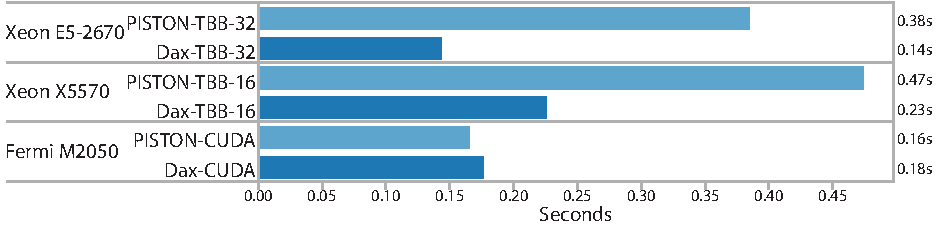
\includegraphics{images/TimingThresholdNoPointMask}
  \caption{Timing of threshold without output point masking.}
  \label{fig:TimingThresholdNoPointMask}
\end{figure}

Even though Dax adds abstractions that are not used in the PISTON
algorithm, the C++ templates remove most of the overhead making the Dax
algorithm very efficient. In some cases we are even faster than the PISTON
algorithm. This is attributed to a 3D block scheduler that is not available
in the Thrust library used by PISTON.

\subsection{Marching Cubes}

The Marching Cubes algorithm\lcite{Lorensen1987} is a classic scientific
visualization algorithm used to extract the contour surface from a volume
where a field is of a particular specified value. In this algorithm each
cell of the volume is analyzed, and using a table of cases and
interpolations a set of polygons representing the contour in that cell are
produced. Polygons produced in adjacent cells will have coincident points,
and managing these connections is parallel processing is challenging. The
operation of Marching Cubes is similar to that of the threshold algorithm.

\begin{itemize}
\item For every cell in the input data set, we need to first determine how
  many polygons and points will be produced. In the case of Marching Cubes,
  we look in our case table and determine the size of the output.
\item Once we have generated the count array, we need to determine how much
  space to allocate in the output and build indices from either input to
  output or output to input. This is a fairly common task in parallel
  programming, known as stream compaction. The Dax dispatcher performs this
  all internally before performing the following step.
\item Armed with a mapping between input and output, a second parallel
  operation generates the points and cell connections that make up the
  contour. This operation is implemented inside of an interpolated cell
  worklet.
\item We know that polygons generated by independent threads will have
  coincident points. The Dax dispatcher can find these coincident points by
  comparing a topological key (currently the edge it is created on and the
  interpolated distance across it). However, this step is optional.
\end{itemize}

We demonstrate the Marching Cubes algorithm by running it on the example
supernova simulation results on a $432^3$ uniform grid. In our first set of
experiments, we run a version of the algorithm that is isomorphic to what
VTK produces. The results of these experiments are summarized in
Figure~\ref{fig:TimingMCManifold}.

\begin{figure}[htb]
  \centering
  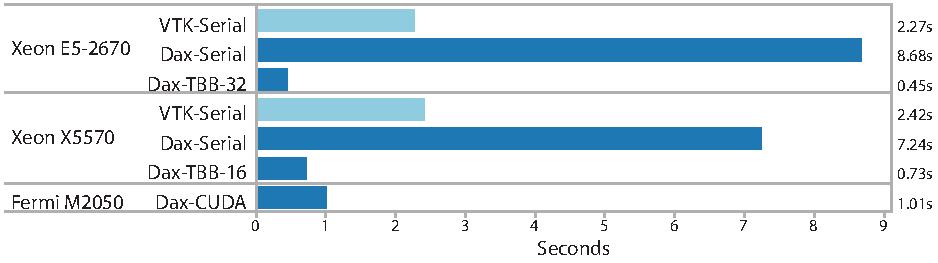
\includegraphics{images/TimingMCManifold}
  \caption{Timing of Marching Cubes when outputting a manifold surface.}
  \label{fig:TimingMCManifold}
\end{figure}

We note that the serial version of the Dax algorithm is slower than that in
VTK, but this is because the VTK contour algorithm is technically not
Marching Cubes. It uses a different algorithm called Synchronized
Templates, which uses the nature of the uniform grid structure to remove
redundant computation and share coincident vertices. However, Synchronized
Templates only works on this type of uniform data, and there is no known
way to parallelize the algorithm. Thus, when Dax is run in parallel it can
outperform the VTK version.

As previously stated, the final step of the interpolated cell method, where
coincident points are merged, is optional. In our second set of
experiments, we run the algorithm on the same data set as before, but skip
the coincident-point-merging step to produce a triangle soup instead of a
manifold surface. We compare the algorithm in Dax with an equivalent
algorithm from the PISTON project. The results of these experiments are
summarized in Figure~\ref{fig:TimingMCSoup}.

\begin{figure}[htb]
  \centering
  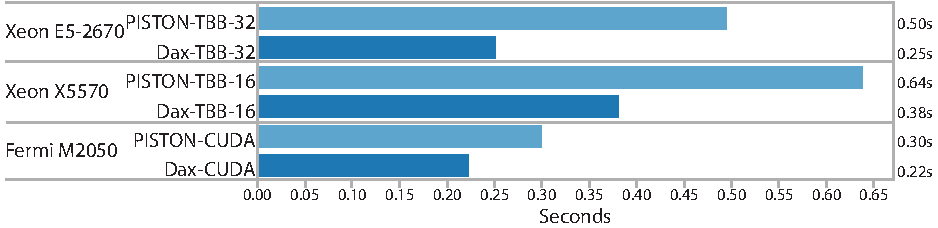
\includegraphics{images/TimingMCSoup}
  \caption{Timing of Marching Cubes when outputting a triangle soup.}
  \label{fig:TimingMCSoup}
\end{figure}

Even though Dax adds abstractions that are not used in the PISTON
algorithm, the C++ templates remove most of the overhead making the Dax
algorithm very efficient.

\section{Future Plans}

We hope to soon start new projects that continue to develop the Dax
framework. There are many avenues of future development we wish to pursue.

\begin{itemize}
\item Integrate more tightly into existing and emerging visualization
  libraries and applications such as VTK, ParaView, VisIt, PISTON, and
  EAVL.
\item Expand the framework to support additional data structures and cell
  types.
\item With the goal to provide a rich collection of commonly used analysis
  algorithms within the toolkit, we will continue work on developing
  worklets (and corresponding work-types) for further algorithms.
\item Begin to use the Dax toolkit on real scientific application problems
  within DOE Office of Science and elsewhere.
\item Facilitate the integration of analysis with simulation by using Dax
  for in situ analysis.
\item Provide a more formal categorization of visualization algorithms and
  behavior in massive parallelism.
\end{itemize}
